\section{Literature Review}

\subsection{User Interface Design}
Having read different articles relating to Human Computer Interaction components, several factors have been identified that directly link to improving interfaces of mobile applications.  Some of these are the use of graphics, colour, font and other effects.  \\
\textbf{Colour} is one of the main attributes and it covers many different areas including background, text colour and visual effects.  Lets first consider background and text colour.  There is a lot of different opinions on this topic; a lot of people will lean towards a light background with dark text.  Dark backgrounds (dark designs) are becoming very popular now and add a creative and elegant appeal to the app.  This is not something that can be left to preference.  There are situations when dark backgrounds suit the app and there are situations when a light background is preferred.  An app with lots of reading is better off having a light background with dark text.  A recent survey was taken on this area and 47\% prefer light background because it aids with \emph{readability}.   Another 10\% said they prefer dark backgrounds with 36\% saying it just depends on the function of the app [0].  With our app in mind, we are not so hung up on readability but eye fatigue.  We want the user to be able to use the app in any conditions whether it be during the day, night, in unilluminated rooms (bars and nightclubs) or illuminated rooms.  With this criteria in mind, we need to consider something that has not too high-contrast.  We do not want a full white on full black or vice versa.  We can use dark grey with off white and this will prevent the eyes burning out.  One final note to make; darker backgrounds tend to use less battery.  A test was carried out on an AMOLED screen and the results showed that `mostly' white background use 1/3 more battery than black backgrounds [1].  Another test was carried out on a Nokia Lumia 720 (with WVGA IPS screen) and this used 6.37\% more battery having a white background compared to dark background [2].  \\
Now if we have the dark grey background, we need to consider other colours to use with the app.  Blue is usually a popular colour of choice (the world's favourite) [3].  Blue is the colour of the intellect and the mind.  However, blue can be difficult to see on certain backgrounds as it tends to blend in.  This is actually to do with our eyes.  There are fewer photoreceptors that react to blue compared to other colours and they are not in the centre of the retina because it is sometimes hard to distinguish.  \\
Lets consider another colour; orange is included in Ubuntu's colour palette as they believe it signifies a community feeling.  There are many other descriptions of orange - it is classified as a warm colour, it radiates warmth and is often associated with energy, happiness, attraction, stimulation and comfort [4].  We want our app to have a community like feeling.  This is an app for the public where they can talk through the language of music.  Two other interesting words here are \emph{attraction} and \emph{stimulation}.  Ultimately we want users to be attracted to our app, enjoy their experience and to keep using it.  Although colour won't have too big an emphasis on this, a well designed app can and colour plays a part in this.  Therefore orange seems to be a good colour choice.  
Colour can also used to convey information through visual recognition.  A colour like green means on, safe, valid etc while red means off, danger, invalid etc.  We can make use of these colours in our app to provide information to the user.  \\
Talking of colour, one of the most important thing to remember is to not use too many different colours.  We want to keep the colour scheme minimal.  A busy colour scheme will obscure the dark background as the contrast will be too sharp.  Therefore we shall stick with 2 different colours and a background colour.  \\

\textbf{Font} is another important consideration.  It is important to make sure the selected font is clean, crisp and works well with colours we have chosen.  There are several areas to consider here; the first being weights.  If we want to try and create contract and a visual hierarchy within the app, we can consider different weights such as light, normal, italics, bold and extra bold.  Legibility is also important due to the number of small scree devices there are currently on the market.  If we use a font that is hard to read when it is smaller, then our app design has a serious flaw.  Therefore it is important to use a \emph{sans serif font}.  This type of font does work well with a dark background.  
he trick, though, is to put only larger text in serif fonts, so that the extra white space floods around each character and makes the text very legible.  \\
There are several other key considerations.  Consistency; the app should be as consistent as possible with commands and menus containing the same content and format.  If there are buttons or features designed on one part of the app that act in a certain way, then if this button/feature appears somewhere else, it should act the same way.  The app must be navigable in the sense that we can manoeuvre between the different pages.  Any messages that are displayed (toast notifications etc) should be descriptive and helpful.  Simplicity is also very important and ensures the user will keep coming back to the app.  Many useful apps have been created over the years yet people do not come back because they find it awkward to use or they find it complicated to use.  An example of this is Bump.  When this was first released, it had features to transfer music, photos, contact information other documents and recommended apps.  But due to its complicated nature, it was slated and users abandoned it.  When the creators re-developed the app with simpler page layouts, the app became easy to naviaged and simple to understand.  That is when its potential was realised and now has been downloaded millions of times.  

\subsection{App frameworks}
There are numerous different frameworks available for us to use in order to create the client side app that users will interact with.  \\
First of all, there is \textbf{PhoneGap}.  PhoneGap allows users to develop hybrid mobile device applications using HTML, CSS and JavaScript.  A hybrid application is one where it is neither a native mobile app (as layout rendering is done via web views instead of a platform native UI framework) nor a pure web-based app (because they packaged as apps for distribution and have access to native device APIs).  PhoneGap works across multiple platforms (iOS, Android, Windows etc.).  However, any app created using this can be slightly unresponsive compared to fully native ones.  There has also been reports that bugs can pop up on specific devices, something we don't want whenever we consider the UK operating system split is 49.7\% android and 42.5\% iOS with the remaining percentage covering Windows, Blackberry and others [4].   \\
Two other frameworks we could use would be \textbf{Eclipse} and textbf{X-code}.  Eclipse creates apps that look and feel professional with the help of the components contained in the SDK.   However, this only produced android apps, thus leaving out all iOS users.  Eclipse is also Java and not JavaScript therefore the skills required are slightly different.    X-code has an amazing UI editor alongside other different development tools that make it easy to create effective and well connected interfaces.  The environment also allows for easy testing and easy release of the app.  However, this produces only iOS app's therefore we are eliminating the android section of the market as well as the others.  X-code is also only available on Mac, therefore we cannot develop it using windows or Linux.  Finally, X-code doesn't use Java or JavaScript, but Objective-C and at the moment, none of us have developed with this.  \\
\textbf{Ionic} is one of the newer frameworks for app development.  Essentially, Ionic is a wrapper around the Cordova framework that comes with a bunch of very powerful CLI (command-line interface) tools - suits some of us more than others.  It has been built on top of AngularJS (from Google) where angular provides an application structure with Ionic providing the User Interface.  The two are harmonious with Ionic providing angular directives for its own components.  This means that certain features can be created with very simple HTML code.  Ionic also makes use of Bower and NPM and having all these popular tools and frameworks surrounding it, makes it a popular choice.  The creators of Ionic said they have focused on performance.  In doing so, they have brought about simplicity - it keeps a flat, clean simple and powerful UI without unnecessary rendering of rounded corners etc.  This fits in with our idea of the app; we want something simple and clean as this will result in a better user experience which will entice the user to use it again.  

\subsection{Effects of Music}
Music comes in very different forms and covers many different genres.  This leaves it very hard to play music that suits most or all kinds of customers.  According to ``Which'', its not actually the music we like that grabs our attention but its the music we don't like that we notice most.   Therefore, we don't want people to be listening to music they don't like for one main reason; it will annoy them and potentially make them leave the facility.  \\

Music has a lot of power; it moves people of all cultures.  Unfortunately, it is not understood as to why listening to music triggers such a rewarding experience but through brain scans, it seems songs trigger the same brain flooding (with dopamine) as food and sex.  This reaction then causes the Nucleus Accumbens to communicate with the temporal gyrus [7].  This essentially causes us to register memories; we have a likeness to remember the fond memories with links of music and sounds.  Having this knowledge, we can essentially use this to stimulate customers; happy customers drawing on happy memories will result in many different activities and these should be mainly positive ones for the shop, whether it be more purchases or decisive purchases.  \\

How music is played also has an effect on our activities within a shop.  There have been several different studies carried out over the years linked to how volume, speed and type of music effects our behaviour.  For instance, the louder the music, the more likely it is that people will spend less time in that shop [8].  There are cases when this is a good thing; both for the customer and for the business.  Lets consider a supermarket.  Before we make our way to the supermarket, we have a fairly good idea of what we want.  Therefore we are not actually going to spend any less money if we are fast and efficient compared with spending more time in the store.  Its good for the customer because we will have more time to spend on other activities and its good for the business because their stores do not become bunged and they should in essence have a steadier stream of customers.  \\
Slower music will result in customers spending more time in store and hopefully an increase in purchases [8].  This type of scenario is what businesses want when customers come for a look around e.g. cloths, furniture, jewellery and coffee shops etc.  The customer may not have had the intention of making any purchases but the slow music changed their brain activity that resulted in a purchase they didn't intend to make.  Even in coffee shops, it may result in the customer(s) grabbing another coffee before leaving. \\
Listening to the wrong type of music can make people believe they have been somewhere longer than they have.  Something like this will force the customer to leave the store, maybe even before they have purchased anything.  Therefore having the right type of music playing is essential to keep the customers in the store long enough to make sure they makes purchase.  There is no better way of doing this than allowing the customer to have a say in the music they listen to. 

\subsection{\textbf{Competitors}}
We have taken a look at other apps and services on the market and feel that nothing matches our idea. The closest service available is from \textbf{Sonos}. Sonos is a smart system of speakers and audio components that unite your digital music collection in one app and can then be controlled from any device. The rise of digital music has allowed for us to bring our music wherever we go, through media such as iPods, MP3 players etc. However, there hasn't been the same advancements in terms of systems that don't move around. `Wireless' is the word that comes to mind when thinking of a solution. It is now possible to stream audio to a wireless device (speaker) and without compromising on the sound quality. Sonos provides the user with the ability to play music from a device wirelessly anywhere in the \textbf{home}. However, there are two issues with this; it is only available for the \textbf{home} and the consumer needs to purchase expensive \textbf{hardware}. The cheapest speaker available for purchase is \pounds169. If you are a music-orientated person, you may wish to purchase their high-end hardware which can cost up to \pounds1200. Unfortunately, Sonos do not support other wireless speakers. An adaptor can be purchased to allow these to be connected to their system, the \emph{Connect} device, but this costs \pounds279.  

\textbf{Pure} have also moved into this market where they provide wireless speakers and hardware for \emph{wireless music} in the \textbf{home}. They also allow you to purchase hardware to link your current speakers with their system at \pounds69.  This is much cheaper than Sonos but is still quite expensive. It allows the consumer to wirelessly play their music from any music app or streaming service they want. \textbf{Bose} also provide a very similar service to Pure, but the hardware costs are more expensive.

From this, we can see that there are no services available for the wireless sharing of music outside the home. Our app would unite music into anybody's daily routine, whether this is at the office, coffee shop, restaurant as well as the home. We also want to make sure that no expensive costs are applied.
Competitors can appear at anytime during the development of a project, so it is important that we keep looking for emerging competitors and that we can identify how our product is unique to theirs. 

\subsection{\textbf{Music Sources}}
In today's market, there are many music sources available to an individual. We have virtual music from services such as `Spotify', `Google Music' and `iTunes' as well as physical music on `iPods', `MP3 players' and other hardware devices. \\

\textbf{Spotify} is a music streaming service that offers access to a library of over 20 million music tracks with over 40 million active users. It is available across 58 markets including the UK, USA, France, Germany, Hong Kong and Argentina. It is available on iOS, Android, Windows phone as well as PC and Mac. One chain that is affiliated with Spotify is Costa. Costa have their own playlist that people can access from their device. \\
\textbf{Google Music} is another streaming service and offers the same service as Spotify. Again, they have a large library of songs (around 18 million) and the service is available in over 57 countries on all Android devices as well as web browsers. \\
\textbf{Auracle Music} is a custom streaming service that delivers the best background music through the internet.  This allows you to tailor the music you have playing to suit your needs.  At the moment, this system contains over 30 different licensed music channels with a whole host of music making it compatible with this project.  The top advantage of this is actually the fact that it is for commercial use.  This therefore means we can use it alongside Choona and not require any further licenses.  \\
A year ago, Apple's \textbf{iTunes} accounted for 75\% of the digital music market and with a huge 575 million active users. Although this may have decreased slightly in the last year, that is still a large user base. As well as general users, Starbucks is affiliated with iTunes and use this service to hand-pick and play music throughout their stores. The idea of allowing customers to put forward their music preference may be of interest to a chain like Starbucks amongst others. 
The issue with iTunes is that all the music has to be purchased before it can be listened to.  There is no monthly subscription fee where you can listen to as much or as little music as possible.  Apple are however brining out their own music streaming service; called \textbf{Beats Music}.    
The above figures suggest that the music streaming industry is vast and that music is a part of many people's lives. Coffee shops have integrated these sources and music into their environment, but without the customer interaction. Choona would provide this interaction. Over the course of this project, we shall identify more sources because having more sources creates a larger user base as well as a better music library. We shall look at how the different sources work to try and make sure we have adaptors in place that can cover the wide variety of sources available. 

\subsection{\textbf{Legal Issues}}
With this type of app, there are certain laws and legislation in place that have to be adhered to in order to play music in public.  
\subsubsection{Public Performance License}
    Music playing for customers or staff through media such as radio, MP3, TV etc. is considered a \emph{public performance}. The \emph{Copyright, Designs and Patents Act 1988} means that an agreement is needed from the copyright owner before the material can be played in public. A music license (PPL) will grant this agreement. In most cases, a license is required but there are a few instances when one is not required. One example of this is where PRS  artists have waived their rights. PRS for Music represents the rights of over 100,000 artists in the UK.  It provides licensing to organisations to allow the playing, performing and availability of copyright music on behalf of the artists and overseas societies.  The royalties are distributed fairly and efficiently.  Another example is a hotel, guest house or B\&B that has fewer than 25 rooms with no areas open to non-residents. 
    Any business such as a coffee shop, bar or gym that plays recorded music in public will legally require a PPL. The likelihood of our service being used in places that don't have a PPL and require one is small.  Most coffee shops, restaurants, gyms etc. will already have the license in place.  It will be work places deciding to implement our service that will have to go about retrieving a PPL.\\
The costs vary depending on the facility and how the music is used.  Cafe's, restaurants, pubs and bars are charged based on the area size, so the smaller the area, the smaller the fee.  This is an annual fee and ranges from between around �130 to �325 per year [6].  The reason the fee is not too large is because the music is just background noise and therefore it is not the main attraction.  In some establishments, they may not play background music and so if they wanted Choona, they will have to apply for the license.  Ultimately, it will be there decision as to whether they decide to take on this extra annual fee; maybe Choona can promote them enough to gain extra sales thus warranting its purchase.    \\
\textbf{Retail shops} too have to pay a fee and again this is based upon the area size of the store.  These range anywhere from around �130 to �220.  A lot of retailer space does not have music in the bacground and so they will need to judge whether or not they want to take on Choona and the required licenses they would need. It is all about whether or not Choona as a service will provide enough benefits over the costs needed.  If the store already has a license in agreement, then the integration of Choona should be simple.  \\
\textbf{Nightclubs} have a different payment scheme; they have a standard fee to pay and on top of that, they pay an additional cost (for each night of entertainment) that is calculated depending on the number of customers (population size) and the number of hours the music will be played [6].  Therefore fees can escalate enormously over a year long period.  This though however would not make any difference for them; they will have to pay these fees regardless of whether Choona is integrated or not therefore integration should be simple and straightforward.  
There are tables highlighting these costs for the different premises and these are available in the Appendix.  
      
\subsubsection{Entertainment Licensing}   
Introduced on 6 April 2015, this licence may need to be acquired by businesses, organisations and even individuals who want to provide entertainment.  This entertainment can cover more than music but for this project, we only want to consider the instances when the entertainment revolves around the playing of music or the performance of music.  This license will apply to places such as night clubs, live music venues (concerts) and large indoor arena's.  \\
Below are the set of conditions where if any are met, a license is required:
\begin{itemize}
\item Entertainment is provided between 11pm and 8am
\item Amplified live/recorded music performed to an audience greater than 500 people
\item Recorded music played to an audience on premises where the sale of alcohol is not licensed.
\end{itemize}
Essentially this covers bars, nightclubs, concerts and other different use cases for Choona.  The fees have been laid out in figure \ref{fig:license_prices}.\\ 

\begin{minipage}{\linewidth}
\centering
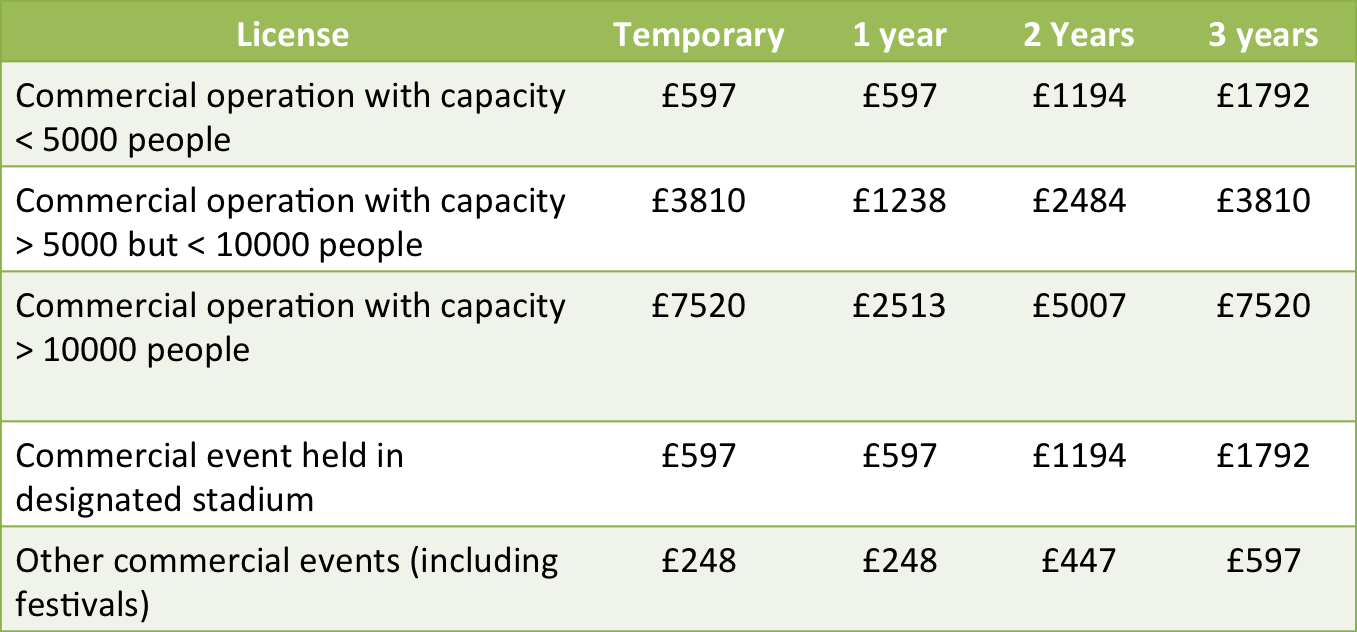
\includegraphics[width=0.8\textwidth]{./img/table_license.png}
\captionof{figure}{The pricing scheme [5]}
\label{fig:license_prices}
\end{minipage}\\

The prices vary somewhat and for the larger events and locations, these prices may not be too much of a concern.  However, when it comes to smaller venues, they may be reluctant to pay the fee.  The process itself in order to get a license, an application is to be submitted.  The application can be considered for a period of 6 months before a decision needs to be made.   This is not a short process and therefore if Choona is to be implemented in certain establishments, the appropriate amount of notice needs to be given so the license can be granted.  

\subsubsection{Music}
At this current moment in time, Spotify is for personal use only.  Therefore we cannot make use of Spotify as a commercial source with it stating in their terms and conditions thats ``Anywhere you need a license to play music, you are not allowed to use Spotify''.  Obviously this is a big issue and something that has to be considered deeply.  There are some small services out there that do allow for commercial use of music streaming (something like Auricle Music) but these are not on the same level as Spotify, Google Music etc.  \\
\textbf{Beats Music} is also for personal/private use only.  There is slight leeway here because unlike Spotify, there allow for commercial use if the user is a curator.  In there case, a curator is someone who has a customised profile page that contains authentic postings and curated playlists.  This will have to be verified with Beats Music.  This could actually allow Choona to create this type of profile and eventually make use of this streaming service as the source.  

\subsection{Geolocation}
\textbf{Geolocation} is a technology solution used to identify the real-world geographic location of an object.  Geolocation makes it possible, from a device connected to the Internet, to obtain various types of information in real time and locate it on the map with high accuracy at a given point in time. 
Many different methods can be used to collect this data but for the purposes of this app, it will be through mobile phones (users device containing the app) and IP addresses (for the Choona service end).  \\
The idea behind geolocation within this project would be to connect the user to the Choona system within their location automatically or show the different Choona locations within their geofence so they can choose which one they want to connect to.  In doing so, we are highlighting Choona locations that are within range only thus limiting the search area and making life simpler for the user.  There are several advantages to Geolocation.  First of all, we can have \textbf{targeted adverts}.  For both the customer and the business running Choona, more locally-targeted adverts can create a better app experience.  Customers will get adverts related to their location and not just any old adverts thus the experience will feel less spammy.  For the businesses, they can use this space to advertise new products, special offers in order to improve sales and custom.  \\
Secondly, Geolocation can help improve user profiles.  We can understand exactly where a user is in terms of activity and thus we use this to promote new app features or create different features based on user preferences.  Things to consider here would be algorithms that automatically indicate songs you can play based on previous songs you have added to playlists.  We can also use this to send push notifications; the sending of messages that could be linked with Choona in general or a specific Choona location.  It is reasonably simple to implement the basic functionality of Geolocation on the app side with use HTML and JavaScript needed but to get it working with the backend will require considerable work and time to make it effective and consistent. 

\subsection{NFC}
Near-Field Communication (NFC) is a form of short range wireless communication (4cm or less to launch a connection) allowing for radio communication and the passing of data packets between two devices, or smart tags that work with NFC. NFC is an advancement to RFID systems because it allows for two-way communication. This two-way communication can then be used for authentication purposes or data exchange. \\
At the moment, not all devices support NFC and it is suggested around 20\% of phones worldwide will have NFC capability by the end of 2014. This figure is set to increase dramatically over the next five years meaning more devices will have the capability and more users will be familiar with the technology. This widespread reach of NFC phones could mean one day that NFC tags become as common as bar codes, so it makes sense to make use of this technology.\\

Using NFC tags with a mobile device, a user could access the playlist at their current location without the need to search for it. The idea is very durable as NFC tags are small and cheap enough to integrate anywhere. They do not need a power source but instead draw power from the device that reads them. \\

\subsubsection{Viability}
With NFC, it is unfortunate that apple devices cannot use it.  Some do have NFC functionality but this is just for the purpose of `Apple Pay' and nothing else.  Almost all android devices currently have NFC functionality that can be used by the apps themselves.  NFC tags or stickers are extremely cheap; around �1 per tag.  In bulk purchases, this will decrease dramatically.  They are extremely easy to encode through a NFC enabled device and allows for protection to stop it being changed by unauthorised user.  If we were to adapt the use of NFC, the business themselves should be able to encode the tags themselves.  It may be an idea to have a tutorial available where the business just needs to follow the small number of steps involved.\\
    